\pdfoutput=1
\documentclass{article}

\usepackage{arxiv}
\AtBeginDocument{\raggedbottom}

\usepackage[utf8]{inputenc}
\usepackage[T1]{fontenc}
\usepackage{courier}
\usepackage{amsmath}
\usepackage{amsfonts}
\usepackage{microtype}
\usepackage{booktabs}
\usepackage{graphicx}
\usepackage{xcolor}
\usepackage[numbers,sort&compress]{natbib}
\usepackage{hyperref}
\usepackage{url}
\usepackage{caption}
\captionsetup{font=small,labelfont=bf}
\usepackage{enumitem}
\setlist{itemsep=2pt,topsep=4pt}
\usepackage{float}

\hypersetup{
  colorlinks=true,
  linkcolor=blue!50!black,
  citecolor=blue!50!black,
  urlcolor=blue!50!black,
  pdftitle={Readmission Models Discriminate Worse for the Oldest Patients},
  pdfauthor={Archit Bhatia},
  pdfkeywords={subgroup evaluation, hospital readmission, algorithmic fairness, age, pre-registration, clinical machine learning}
}

\newcommand{\ci}[2]{\,\mbox{[#1,\,#2]}}

\title{Readmission Models Discriminate Worse for the Oldest Patients: A Pre-Registered Patient-Level Audit of the Diabetes 130-US Hospitals Benchmark}

\author{
  Archit Bhatia \\
  Plaksha University\\
  Mohali, Punjab, India \\
  \texttt{archit.bhatia.pg26@plaksha.edu.in}
}

\renewcommand{\shorttitle}{Age Gap in Readmission-Model Discrimination}
\renewcommand{\headeright}{Preprint}
\renewcommand{\undertitle}{Preprint}
\date{}

\begin{document}
\maketitle

\begin{abstract}
Aggregate discrimination metrics can hide subgroup failures. I ask whether a standard 30-day readmission model discriminates equally well across age and, if not, why. On the UCI Diabetes 130-US Hospitals data (first encounter per patient, deaths and hospice discharges excluded; $n = 69{,}990$), logistic regression reaches an overall AUC of 0.648, but 0.647 for patients aged 40--59 and 0.603 for those aged 80 and over: a gap of 0.044 (paired patient-level bootstrap 95\% CI 0.021 to 0.066). LightGBM gives 0.036 (0.013 to 0.059). An encounter-level analysis roughly doubles the gap, mostly because repeat admitters are easy to predict, not because of train--test leakage. Following an analysis plan committed before any result was computed, I show that the remaining gap is not explained by outcome rarity, outcome definition, sample size (parallel learning curves; the gap persists at equal training size) or model capacity (four model classes, including explicit age-by-feature interactions). It is confined to the region of feature space occupied mainly by the oldest patients. Band-specific models, reweighting, finer diagnosis codes and geriatric-syndrome flags do not raise their AUC. Calibration-in-the-large holds at every age, but the calibration slope for the 80+ band is 0.72 (0.62 to 0.82). I conclude that the gap reflects missing information in these features rather than a deficiency of the learner, and that results on this benchmark should be reported with age-stratified discrimination and calibration.
\end{abstract}

\keywords{Subgroup evaluation \and Hospital readmission \and Algorithmic fairness \and Older adults \and Pre-registration \and Clinical machine learning}

\section{Introduction}

Readmission risk models are usually summarised by a single AUC. If discrimination is materially worse for an identifiable group, the model's ranking of patients is least trustworthy where it is used, and the aggregate hides this. Older adults have the highest readmission rates and the most to gain or lose from risk stratification.

This study grew out of a preliminary analysis I carried out as an unpublished course project. That analysis used an encounter-level design with a single random split. It found a large AUC gap by age that survived a stronger model, and proposed an explanation based on diagnosis complexity, which direct tests did not support and which was retracted. That left a finding without an explanation. Here I replace the preliminary analysis with a pre-specified, patient-level study (the methodological differences are listed in Appendix~\ref{app:changes}) that asks three questions:
\begin{enumerate}
  \item Is discrimination lower for the oldest patients once the analysis is done at the patient level?
  \item If so, is the gap explained by cheap factors (base rate, outcome definition, case mix, discharge destination), by variance (too little data), or by bias (insufficient model capacity)? Or does it persist after all of these, pointing to features that carry less information about the oldest patients?
  \item Does any straightforward intervention close the gap?
\end{enumerate}

\paragraph{Contributions.}
\begin{enumerate}
  \item A pre-registered, patient-level estimate of the age gap on a widely used benchmark, with paired confidence intervals for the difference.
  \item Evidence that about half of the gap in the usual encounter-level analysis comes from repeat admitters, not from leakage.
  \item A decomposition of the remaining gap: it is not base rate, outcome definition, sample size or model capacity, and it is confined to the elderly-specific region of feature space.
  \item A null result: band-specific models, reweighting, finer ICD-9 codes and geriatric-syndrome flags do not close it.
\end{enumerate}

\section{Data and methods}

\paragraph{Data and cohort.} I use the UCI Diabetes 130-US Hospitals dataset \citep{uci2014}, which covers 1999--2008 and contains 101,766 encounters from 71,518 patients. I follow the cohort definition of its authors \citep{strack2014}: I exclude encounters ending in death (discharge codes 11, 19, 20, 21) or hospice discharge (13, 14), then keep each patient's first encounter. This leaves 69,990 patients; \citet{strack2014} report 69,984, and I have not traced the six-patient difference. The outcome is readmission within 30 days (8.98\%). Table~\ref{tab:cohort} gives the band sizes.

\begin{table}[h]
\centering\small
\caption{Primary cohort by age band.}
\label{tab:cohort}
\begin{tabular}{@{}lrrr@{}}
\toprule
Band & $n$ & Readmitted $<$30 days & Rate \\
\midrule
$<$40 & 4,500 & 300 & 6.7\% \\
40--59 & 19,179 & 1,386 & 7.2\% \\
60--79 & 33,440 & 3,232 & 9.7\% \\
80+ & 12,871 & 1,367 & 10.6\% \\
\midrule
All & 69,990 & 6,285 & 9.0\% \\
\bottomrule
\end{tabular}
\end{table}

\paragraph{Models and features.} I compare two models: logistic regression (LR), with one-hot categoricals and standardised numerics, and LightGBM \citep{ke2017} with 300 trees, learning rate 0.05 and 31 leaves. Both use the same 43 features: 9 numeric fields, including age as the bucket midpoint, and 34 categorical fields covering demographics, admission and discharge codes, medical specialty, the three ICD-9 diagnosis codes grouped into nine categories, laboratory flags and the diabetes medication fields. Implementation uses scikit-learn \citep{pedregosa2011}.

\paragraph{Evaluation.} All metrics use out-of-fold predictions from 5-fold cross-validation, grouped by patient and stratified by outcome and age band. The primary estimand is
\[
\Delta = \mathrm{AUC}_{40\text{--}59} - \mathrm{AUC}_{80+}.
\]
The reference band, 40--59, was fixed in the analysis plan. It is preferred to a best-versus-worst comparison for two reasons: the youngest band is the smallest (4,500 patients, 300 readmissions) and its two lowest 10-year buckets contain almost no positives (3 and 26; Table~\ref{tab:decades}), so its AUC is the least precise; and choosing the comparison after seeing which band scores highest would inflate the gap. The maximum-minus-minimum AUC across all four bands is reported as a pre-specified secondary estimand.
Uncertainty comes from a paired patient-level bootstrap with 2,000 replicates. Each replicate resamples patients once and evaluates every band and model on the same resample, so intervals for differences are valid even where per-band intervals overlap.

\paragraph{Pre-registration.} The analysis plan fixed the cohort, bands, estimand, models, features and every decision rule used below. It was committed to the repository before any result was computed. Deviations, mostly added exploratory analyses, are logged with reasons in Appendix~\ref{app:deviations}.

\section{Results}

\subsection{A patient-level analysis halves the gap but does not remove it}

Table~\ref{tab:leakage} and Figure~\ref{fig:cohort} move from the design of the preliminary analysis (A) to the primary cohort (D), one change at a time.

\begin{table}[h]
\centering\small
\caption{Age gap $\Delta$ (95\% CI) under four designs.}
\label{tab:leakage}
\begin{tabular}{@{}llcc@{}}
\toprule
& Design & LR & LightGBM \\
\midrule
A & All encounters, random row-level 80/20 split & 0.076\ci{0.040}{0.109} & 0.068\ci{0.032}{0.100} \\
B & All encounters, patient-grouped CV & 0.069\ci{0.052}{0.087} & 0.063\ci{0.046}{0.082} \\
C & B, deaths and hospice excluded & 0.080\ci{0.061}{0.097} & 0.079\ci{0.061}{0.097} \\
D & First encounter per patient (primary) & \textbf{0.044}\ci{0.021}{0.066} & \textbf{0.036}\ci{0.013}{0.059} \\
\bottomrule
\end{tabular}
\end{table}

In design A, 41.6\% of test encounters belong to a patient who also appears in training. Grouping by patient nevertheless changes the gap little (A$\to$B). The reduction happens when only one encounter per patient is kept (C$\to$D). Repeat admitters have many prior inpatient visits, which makes them easy to predict, and they inflate AUC most in the young bands. In the preliminary analysis, AUC was 0.81 for ages 20--29. In the primary cohort it is 0.70\ci{0.63}{0.76}, while ages 90--99 reach only 0.54\ci{0.50}{0.59} (Appendix Table~\ref{tab:decades}).

In the primary cohort, AUC is roughly flat at about 0.64--0.66 from age 40 to 79 and falls after 80 (Table~\ref{tab:primary}). The gap is stable across five re-randomised CV splits: its standard deviation is 0.002 for LR and 0.004 for LightGBM. The secondary estimand, the maximum-minus-minimum AUC across the four bands, is 0.077\ci{0.042}{0.113} for LR and 0.062\ci{0.031}{0.098} for LightGBM. It exceeds $\Delta$ because the $<$40 band has the highest point estimate, which is also the least precise (Table~\ref{tab:primary}).

\begin{figure}[t]
\centering
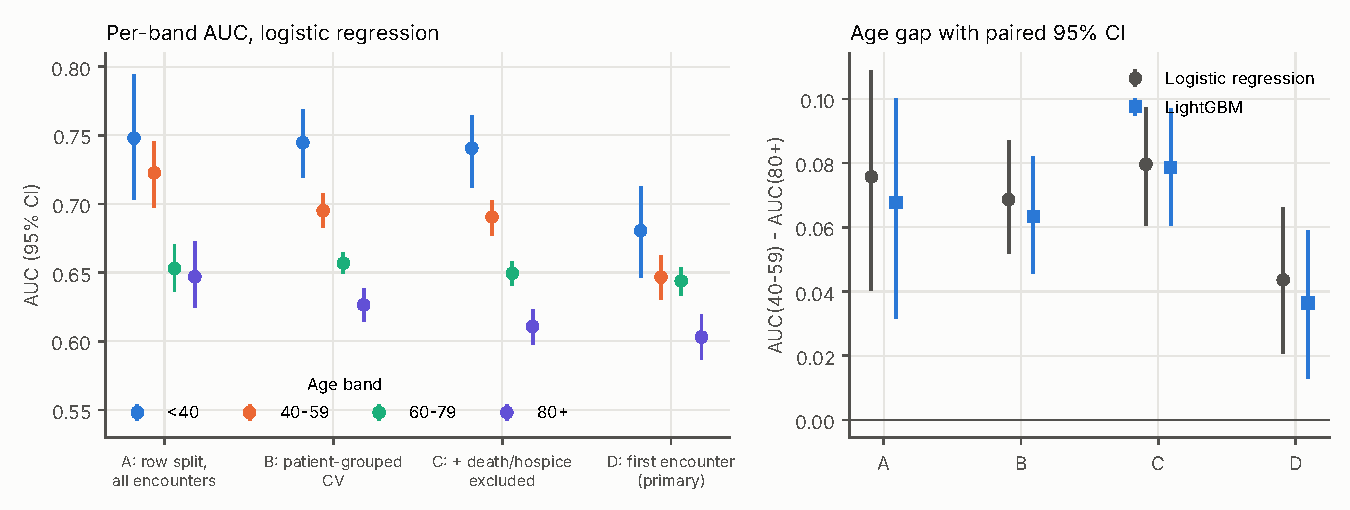
\includegraphics[width=\linewidth]{figures/fig1_cohort_cleaning}
\caption{Left: per-band AUC (LR) under designs A--D. Right: the age gap with paired 95\% CIs. Most of the shrinkage comes from keeping one encounter per patient (C$\to$D), not from grouping by patient (A$\to$B).}
\label{fig:cohort}
\end{figure}

\begin{table}[h]
\centering\small
\caption{Primary cohort: AUC by age band (95\% CI).}
\label{tab:primary}
\setlength{\tabcolsep}{4pt}\footnotesize
\begin{tabular}{@{}lccccc@{}}
\toprule
Model & $<$40 & 40--59 & 60--79 & 80+ & Overall \\
\midrule
LR & 0.681\ci{0.647}{0.713} & 0.647\ci{0.630}{0.662} & 0.644\ci{0.633}{0.654} & 0.603\ci{0.587}{0.620} & 0.648\ci{0.640}{0.655} \\
LightGBM & 0.675\ci{0.642}{0.708} & 0.650\ci{0.633}{0.665} & 0.647\ci{0.637}{0.657} & 0.613\ci{0.597}{0.630} & 0.652\ci{0.645}{0.659} \\
\bottomrule
\end{tabular}
\end{table}

\subsection{Cheap explanations}

\paragraph{Base rate.} Readmission is \emph{more} common in the 80+ band (10.6\% vs.\ 7.2\%), and the two bands have nearly equal numbers of positives (1,367 vs.\ 1,386). Outcome rarity cannot explain the lower AUC.

\paragraph{Outcome definition.} The gap persists when the outcome is redefined. For readmission within 30 days versus never readmitted (dropping later readmissions), $\Delta$ is 0.063\ci{0.040}{0.085} for LR and 0.056\ci{0.034}{0.076} for LightGBM. For any readmission versus never readmitted, it is 0.044\ci{0.031}{0.055} and 0.035\ci{0.022}{0.047}.

\paragraph{Case mix.} A cross-fitted LightGBM model estimates the probability that a patient belongs to the 80+ band rather than 40--59, using every feature except age. It separates the two bands well (AUC 0.86).
\begin{itemize}
  \item \emph{Pre-specified test.} Reweighting 40--59 patients by the odds of belonging to 80+ (weights truncated at the 99th percentile) does not shrink the gap: $\Delta$ is 0.053\ci{0.018}{0.087} for LR. Middle-aged patients who resemble the elderly are still predicted well.
  \item \emph{Exploratory reverse test.} Reweighting 80+ patients to the 40--59 case mix removes the gap: $\Delta$ is $-0.003$\ci{$-$0.039}{0.034}.
\end{itemize}
The deficit is therefore confined to the region of feature space occupied mainly by the elderly. Overlap is limited (effective sample sizes 3,183 to 3,695), so the reweighted estimates describe the region where the two bands overlap.

\paragraph{Discharge destination.} 31.5\% of 80+ patients are discharged to a skilled nursing facility, against 3.6\% of 40--59 patients. Within each destination the gap shrinks, and its CI includes zero for home discharges (LR 0.021\ci{$-$0.015}{0.057}) and for skilled nursing (0.022\ci{$-$0.051}{0.092}). These within-stratum tests are underpowered.

\paragraph{Calibration.} Calibration-in-the-large is close to zero in every band, and the spread of predicted risk is not narrower for 80+ (standard deviation of the predicted logit 0.52 vs.\ 0.48). The calibration slope, however, is 0.72\ci{0.62}{0.82} for 80+ against 1.00\ci{0.92}{1.09} for 40--59. The model separates elderly patients as confidently as younger ones, but those differences in predicted risk overstate the true differences in risk.

\subsection{Decomposition: not variance, not capacity}

\paragraph{Variance.} The learning curves for the two bands are parallel (Figure~\ref{fig:lc}). Going from half to all of the training data raises AUC by 0.008 for 80+ and 0.006 for 40--59 with LR, and by 0.014 and 0.016 with LightGBM. Neither pattern meets the pre-specified criterion for a variance-dominated gap. The fitted LR asymptotes are 0.611 for 80+ and 0.652 for 40--59. Band-specific LR models trained on equal samples of 12,871 patients reach 0.589 for 80+ and 0.632 for 40--59.

\begin{figure}[t]
\centering
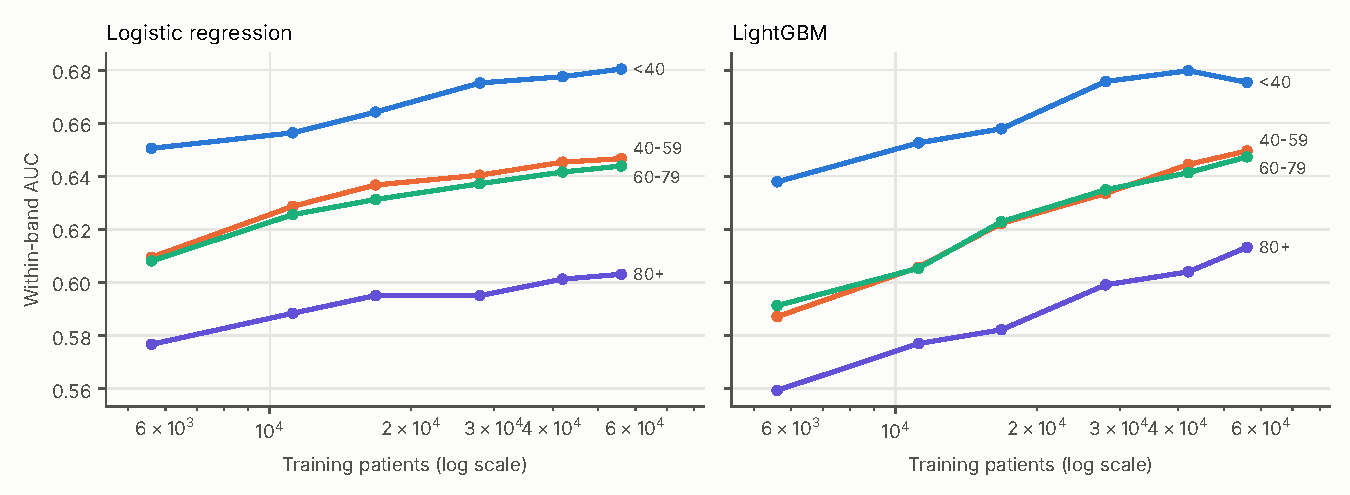
\includegraphics[width=\linewidth]{figures/fig2_learning_curves}
\caption{Within-band AUC as training size grows (pooled out-of-fold predictions, mean of three subsamples). The curves stay parallel, so more data helps every band about equally and the gap persists.}
\label{fig:lc}
\end{figure}

\paragraph{Bias.} Across four model classes, $\Delta$ ranges from 0.036 to 0.048 (Table~\ref{tab:modelclass}), and every paired difference from LR has a CI that includes zero.

\begin{table}[h]
\centering\small
\caption{Model capacity does not move the gap.}
\label{tab:modelclass}
\begin{tabular}{@{}lcc@{}}
\toprule
Model & AUC 80+ & $\Delta$ (95\% CI) \\
\midrule
LR & 0.603 & 0.044\ci{0.021}{0.066} \\
LR with age-band $\times$ feature interactions & 0.597 & 0.048\ci{0.024}{0.070} \\
LightGBM (300 trees, 31 leaves) & 0.613 & 0.036\ci{0.013}{0.059} \\
LightGBM (1,000 trees, 63 leaves) & 0.596 & 0.047\ci{0.025}{0.069} \\
\bottomrule
\end{tabular}
\end{table}

\paragraph{Noise (weak evidence).} Within each band, I fit $k$-nearest-neighbour classifiers to standardised features at matched sample size, as a proxy for how well the features separate outcomes. At $n = 12{,}871$, within-band $k$-NN AUC is lowest for 80+ at every $k$ (for $k = 100$: 0.556 vs.\ 0.582 for 40--59). At $n = 4{,}500$, the 80+ and 60--79 bands cannot be distinguished, so this evidence is weak.

\paragraph{A recording ceiling as a candidate mechanism.} The dataset stores at most three diagnosis codes per encounter, and the diagnosis count is capped at 9. 54.2\% of 80+ patients are at the cap, compared with 37.4\% of 40--59 patients. The diagnosis count carries some signal in the 40--59 band (single-feature AUC 0.56) and none in the 80+ band (0.50). Permutation importance shows the same pattern: discharge destination and prior inpatient visits carry discrimination in every band, while diagnosis-derived features lose importance with age.

\subsection{Interventions: a null result}

No intervention raised AUC for the 80+ band (Figure~\ref{fig:int}). The changes, relative to the baseline model of the same family, were:
\begin{itemize}
  \item band-specific models: LR $-0.007$, LightGBM $-0.036$;
  \item upweighting 80+ patients by a factor of 2 or 5: between $-0.015$ and $+0.001$;
  \item full 3-digit ICD-9 codes and full medical specialty: LR $-0.002$, LightGBM $-0.028$;
  \item eight geriatric-syndrome flags derived from the recorded diagnoses (dementia, delirium, Parkinson's disease, fall-related fracture, pressure ulcer, malnutrition or dehydration, urinary tract infection, pneumonia or aspiration): LR $+0.001$, LightGBM $-0.001$.
\end{itemize}
One variant, LR with 80+ patients weighted by 5, reduced $\Delta$ to 0.029. It did so by lowering AUC for 40--59 (0.647 to 0.631) while leaving 80+ unchanged. I report it as levelling down, not as a fix.

\begin{figure}[t]
\centering
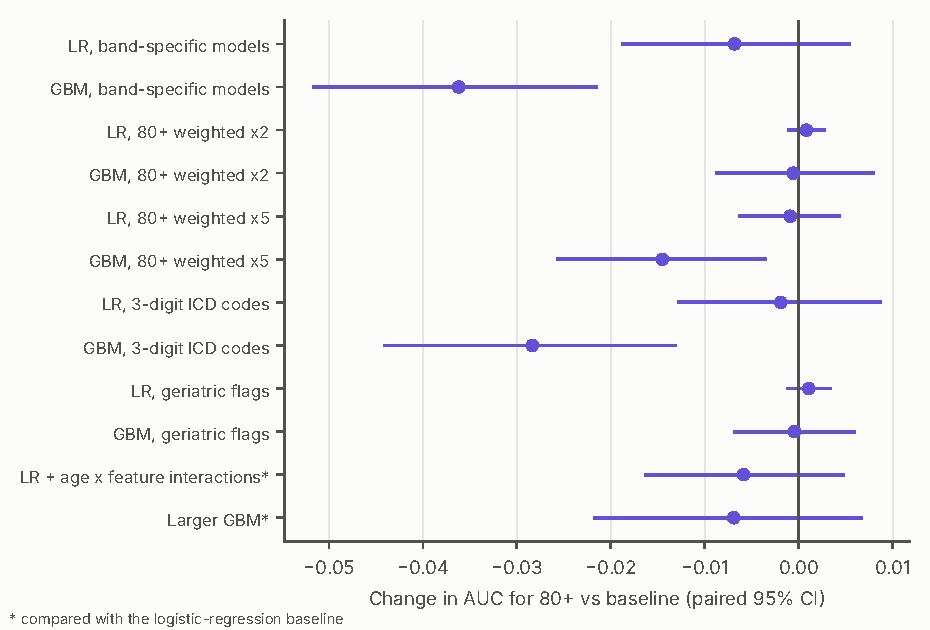
\includegraphics[width=0.78\linewidth]{figures/fig3_interventions}
\caption{Change in AUC for the 80+ band relative to the baseline of the same model family (paired 95\% CIs). No intervention improves it; several LightGBM variants make it worse.}
\label{fig:int}
\end{figure}

\section{Related work}

The closest prior work on this dataset is \citet{alzanbouri2024}. They use the same four age bands and report group fairness metrics (positive prediction rates, false discovery and false omission rates) for several classifiers. They do not report subgroup discrimination (AUC) with confidence intervals, do not describe a patient-level analysis, and do not attempt to explain the differences.

Most other fairness work on this dataset concerns race. The Fairlearn version of the data \citep{fairlearn_diabetes} is encounter-level and bins age as 30 or younger, 30--60 and over 60. That binning merges the band with the deficit (80+) with one without it (60--79). Recent methods papers on the dataset target cross-racial fairness \citep{luxu2026}.

More broadly, readmission models discriminate only modestly. A systematic review found c-statistics from 0.55 to 0.83, with few above 0.70, and noted that functional and social variables, rarely present in administrative data, improve discrimination \citep{kansagara2011}. In older inpatients, frailty and social support add discrimination beyond clinical variables \citep{sokoreli2019,kahlon2015}, consistent with the reading that the 80+ deficit reflects missing information.

Methodologically, the study follows the bias--variance--noise decomposition of \citet{chen2018}. The study is motivated by documented subgroup failures of clinical algorithms \citep{obermeyer2019,seyyed2021}.

\section{Limitations}

\begin{itemize}
  \item \emph{Competing mortality.} Deaths in hospital and hospice discharges are excluded, but deaths after discharge are not recorded. Some elderly patients labelled ``not readmitted'' may have died within 30 days. This adds label noise exactly where the deficit appears, and it is the most important untested explanation.
  \item \emph{Age resolution and confounding.} Age is recorded only in 10-year buckets, and it is confounded with care setting: the case-mix and destination analyses place the deficit where old age and nursing-facility discharge coincide.
  \item \emph{The noise interpretation.} The $k$-NN estimate depends on the feature representation. ``Noise'' here is the explanation left after variance and capacity are ruled out, not a direct measurement.
  \item \emph{External validity.} The data are from 1999--2008, from US hospitals, and cover diabetic encounters only. I have not replicated the result on a second dataset.
  \item \emph{Bootstrap scope.} The confidence intervals treat the out-of-fold predictions as fixed. Variability across re-randomised splits is reported separately (standard deviation of $\Delta$ 0.002 to 0.004).
\end{itemize}

\section{Conclusion}

A readmission model with an overall AUC of 0.65 ranks patients aged 80 and over noticeably worse than middle-aged patients. About half of the gap seen in a standard encounter-level analysis is an artefact of repeat admissions. The remainder survives every check in a pre-specified plan, and more data, more capacity, band-specific models and finer diagnosis codes do not close it. The features in this dataset carry less information about which of the oldest patients will be readmitted. Closing the gap likely requires different data, such as functional status, frailty, social support and post-discharge mortality, rather than a different model. Until such data are available, results on this benchmark should report age-stratified AUCs and calibration slopes alongside the aggregate.

\appendix
\section{Deviations from the pre-registered plan}
\label{app:deviations}
None of these deviations changes a pre-specified estimand, threshold or decision rule.
\begin{enumerate}
  \item The 10-year-bucket table, a secondary analysis, uses a 500-replicate row bootstrap instead of 2,000 replicates.
  \item The reverse case-mix reweighting (80+ reweighted to the 40--59 mix) was added and is labelled exploratory.
  \item The learning curves use 3 subsampling repeats per training fraction instead of 5, because of compute limits. The LightGBM power-law fits reached their parameter bounds and are not interpreted; the pre-specified gain criterion is used instead.
  \item $k$-NN used $k \in \{10, 25, 50, 100\}$ instead of $\{5, 10, 25\}$, because with an outcome rate of 7--11\%, $k = 5$ leaves almost no positives in a neighbourhood. The analysis was run at two matched sample sizes.
  \item Single-feature AUCs, the diagnosis-ceiling check and the geriatric-syndrome flags were added and are labelled exploratory.
\end{enumerate}

\section{Differences from the preliminary analysis}
\label{app:changes}
\begin{table}[H]
\centering\small
\caption{Methodological differences between the preliminary analysis (an unpublished course project) and this study.}
\label{tab:changes}
\begin{tabular}{@{}p{3.1cm}p{5.4cm}p{6.2cm}@{}}
\toprule
Aspect & Preliminary analysis & This study \\
\midrule
Unit of analysis & Encounters (101,766) & First encounter per patient (69,990) \\
Exclusions & None & Deaths and hospice discharges, as in \citet{strack2014} \\
Train/test design & One random 80/20 row split & 5-fold CV, grouped by patient, stratified by outcome $\times$ age band \\
Uncertainty & Separate bootstrap per subgroup & Paired patient-level bootstrap; CI on the \emph{difference} \\
Age groups & Ten 10-year buckets & Four bands fixed in advance: $<$40, 40--59, 60--79, 80+ \\
Estimand & Best vs.\ worst bucket & $\Delta = \mathrm{AUC}_{40\text{--}59} - \mathrm{AUC}_{80+}$, fixed in advance \\
Features & Integer-coded categoricals, raw ICD codes & One-hot categoricals, ICD-9 groups of \citet{strack2014}, top-15 specialty \\
Analysis plan & Developed during analysis & Committed to git before any result; deviations logged \\
Mechanism & Correlation over 9 age buckets (retracted) & Bias/variance/noise decomposition \citep{chen2018} and interventions \\
\bottomrule
\end{tabular}
\end{table}

\section{AUC by 10-year bucket}
\begin{table}[H]
\centering\small
\caption{Primary cohort, LR, AUC by recorded 10-year bucket (500-replicate bootstrap). The two youngest buckets have very few positives.}
\label{tab:decades}
\begin{tabular}{@{}lrrc@{}}
\toprule
Bucket & $n$ & Positives & AUC (95\% CI) \\
\midrule
0--9 & 153 & 3 & 0.451\ci{0.129}{0.937} \\
10--19 & 534 & 26 & 0.678\ci{0.556}{0.789} \\
20--29 & 1,121 & 83 & 0.701\ci{0.634}{0.764} \\
30--39 & 2,692 & 188 & 0.663\ci{0.618}{0.701} \\
40--49 & 6,828 & 506 & 0.635\ci{0.609}{0.660} \\
50--59 & 12,351 & 880 & 0.656\ci{0.635}{0.675} \\
60--69 & 15,689 & 1,415 & 0.644\ci{0.629}{0.662} \\
70--79 & 17,751 & 1,817 & 0.641\ci{0.627}{0.655} \\
80--89 & 11,110 & 1,199 & 0.612\ci{0.595}{0.629} \\
90--99 & 1,761 & 168 & 0.544\ci{0.501}{0.586} \\
\bottomrule
\end{tabular}
\end{table}

\section{Calibration by band}
\begin{table}[H]
\centering\small
\caption{LR calibration in the primary cohort. The slope comes from a logistic recalibration of the outcome on the predicted logit (300-replicate bootstrap CI). The intercept is calibration-in-the-large with the predicted logit as an offset.}
\begin{tabular}{@{}lcccc@{}}
\toprule
Band & Slope (95\% CI) & Intercept & ECE & SD of logit \\
\midrule
$<$40 & 1.17\ci{0.98}{1.40} & 0.04 & 0.008 & 0.49 \\
40--59 & 1.00\ci{0.92}{1.09} & $-0.08$ & 0.007 & 0.48 \\
60--79 & 0.97\ci{0.90}{1.02} & 0.05 & 0.006 & 0.51 \\
80+ & 0.72\ci{0.62}{0.82} & $-0.05$ & 0.016 & 0.52 \\
\bottomrule
\end{tabular}
\end{table}

\section*{Code and data availability}
The data are public \citep{uci2014}. All code, the pre-registered plan with its commit history, the logged deviations and every results table are available at \url{https://github.com/Archit733/readmission-subgroup-audit} (folder \texttt{research/}). A single script, \texttt{run\_all.sh}, regenerates every number and figure in about 25 minutes on two CPU cores.

\section*{Acknowledgements}
AI assistance (Claude, Anthropic) was used for analysis code and drafting. The author reviewed the code, re-derived the headline results independently, and checked every reported number and reference.

\bibliographystyle{plainnat}
\bibliography{refs}

\end{document}
